

\section{Assemblage Smart-Car}
Bij de kick-off van het project is de \gls{Smart-Car} geassembleerd.
De \gls{Smart-Car} bestaat uit de volgende onderdelen: onderkant, bovenkant, sensoren en actuatoren.
\\
\begin{figure}[h]
    \centering
    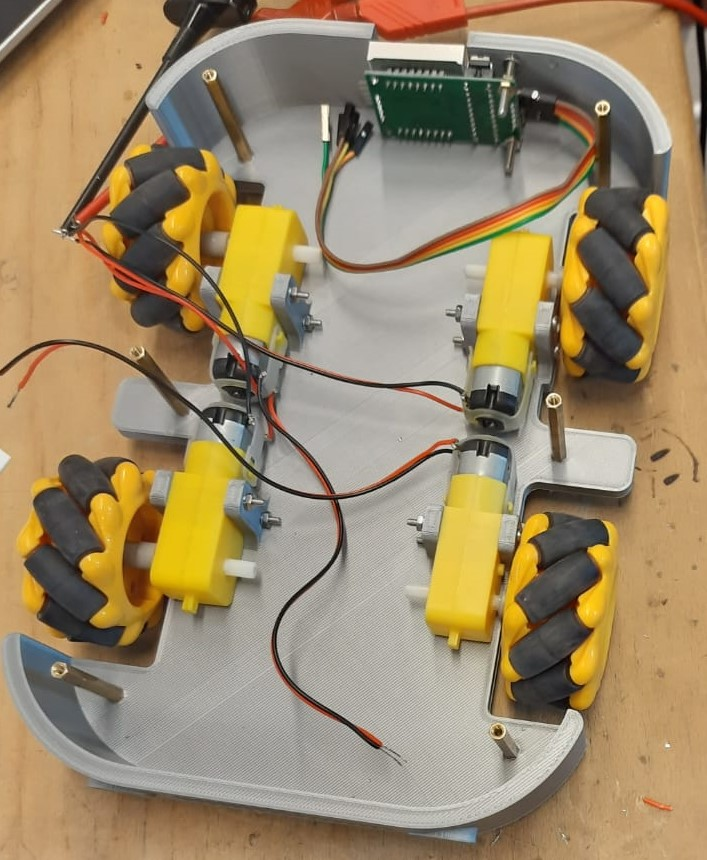
\includegraphics[scale = 0.35]{Media/Figuren/assembleren onderkant.jpg}
    \caption{Onderkant}
    \label{Onderkant-Smart-Car}
\end{figure}
\\
In figuur \ref{Onderkant-Smart-Car} is de onderkant van de \gls{Smart-Car} te zien. Aan de onderkant worden de motoren en de LED-matrix gemonteerd met schroeven en moeren.
\\
\begin{figure}[h]
    \centering
    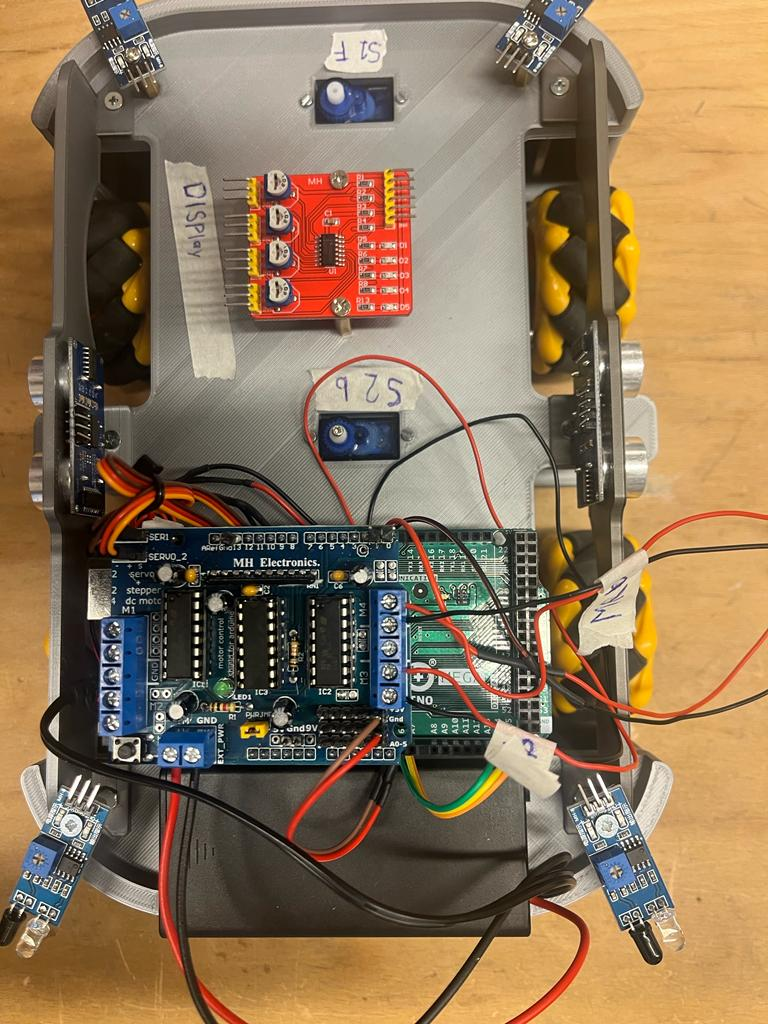
\includegraphics[scale = 0.20]{Media/Figuren/assembleren bovenkant.jpg}
    \caption{Bovenkant}
    \label{Bovenkant-Smart-Car}
\end{figure}
\\
In figuur \ref{Bovenkant-Smart-Car} is de bovenkant van de \gls{Smart-Car} te zien. Op de bovenkant zijn de ultrasonische sensoren,  infrarood sensoren, Arduino Mega 2560 met daarop de motorshield en de servo motoren. Er is voor gekozen om acht infrarood sensoren te gebruiken, zie \ref{Hoofdstuk-IR-onderdelen}. 
\\
\begin{figure}[h]
    \centering
    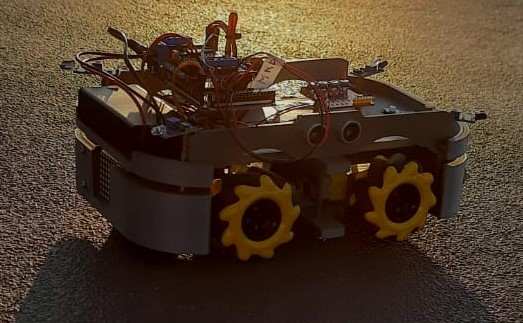
\includegraphics[scale = 0.7]{Media/Figuren/assembleren totaal.jpg}
    \caption{Eindassemblage}
    \label{Eindresultaat-Smart-Car}
\end{figure}
\\
In figuur \ref{Eindresultaat-Smart-Car} is het eindresultaat te zien van de \gls{Smart-Car}, waarbij de bovenkant en onderkant aan elkaar zijn gemonteerd.


\section{Uit welke onderdelen bestaat de Smart-Car en waarvoor worden deze gebruikt?}
De \gls{Smart-Car} bestaat uit verschillende onderdelen, waaronder sensoren en actuatoren. Sensoren zoals infrarood\cite{IR-datasheet}- en ultrasonische sensoren worden gebruikt om objecten te detecteren en afstanden te meten, terwijl motoren worden aangestuurd door een \gls{motorshield} dat bestaat uit een \gls{shift-register} en motor drivers\cite{h-brug}. De negen axis sensor meet de oriëntatie van de \gls{Smart-Car} en wordt momenteel alleen gebruikt om de auto rechtdoor te laten rijden.
\subsection{Sensoren}
\subsubsection{Infrarood sensoren} \label{Hoofdstuk-IR-onderdelen}
\begin{figure}[h]
    \centering
    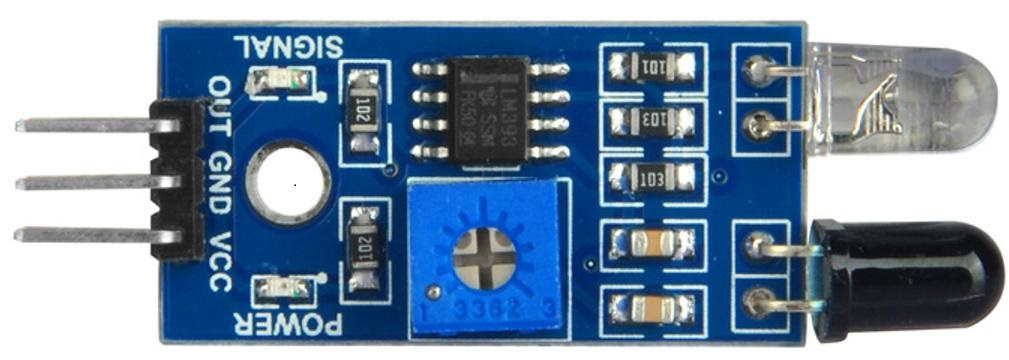
\includegraphics[scale = 0.35]{Media/Figuren/HW-201.jpg}
    \caption{HW-201}
    \label{HW-201}
    \cite{HW-201-hardware} 
\end{figure}
Infrarood sensoren werken door infrarood straling te zenden en te ontvangen. Het zenden gebeurd met een Infrarood led en het ontvangen met een fotodiode. Het is geschikt voor het detecteren van objecten \cite{IR-datasheet}.

In eerste instantie waren HW-201 infrarood sensoren gebruikt voor het detecteren van objecten van 2 tot 30 centimeter. In figuur \ref{HW-201}\cite{HW-201-hardware} is de HW-201 te zien. Voor de eisen van het project is aangegeven dat er vier infrarood sensoren gebruikt moeten worden met in elke hoek één infrarood sensor. De voorste sensoren wijzen naar voren en de achterste sensoren wijzen naar achteren. Door Infra Vroom is er gekozen om vier extra infrarood sensoren te plaatsen, zodat de \gls{Smart-Car} uiteindelijk makkelijker door zijn omgeving kan manoeuvreren. In elke hoek is er één sensor extra geplaatst die naar de zijkant van de \gls{Smart-Car} wijst. Uiteindelijk is ervoor gekozen een ander soort sensor te gebruiken met dezelfde werking, omdat de HW-201 te groot is. De vervangende infrarood sensoren zijn ontworpen door een van de begeleidende docenten en worden alleen voor de \gls{Smart-Car} gebruikt. Deze Infrarood sensoren hebben dezelfde werking als de HW-201 infrarood sensoren alleen is er nu een centrale printplaat in het midden van de \gls{Smart-Car} met in elke hoek een ontvanger, zender en een output pin die op de printplaat kan worden aangesloten. Uiteindelijk is er besloten om de infrarood sensoren te gebruiken om te bepalen of er een blokkade is in de richting waarin de sensor wijst.
\subsubsection{Ultrasonische sensoren}
\begin{figure}[h]
    \centering
    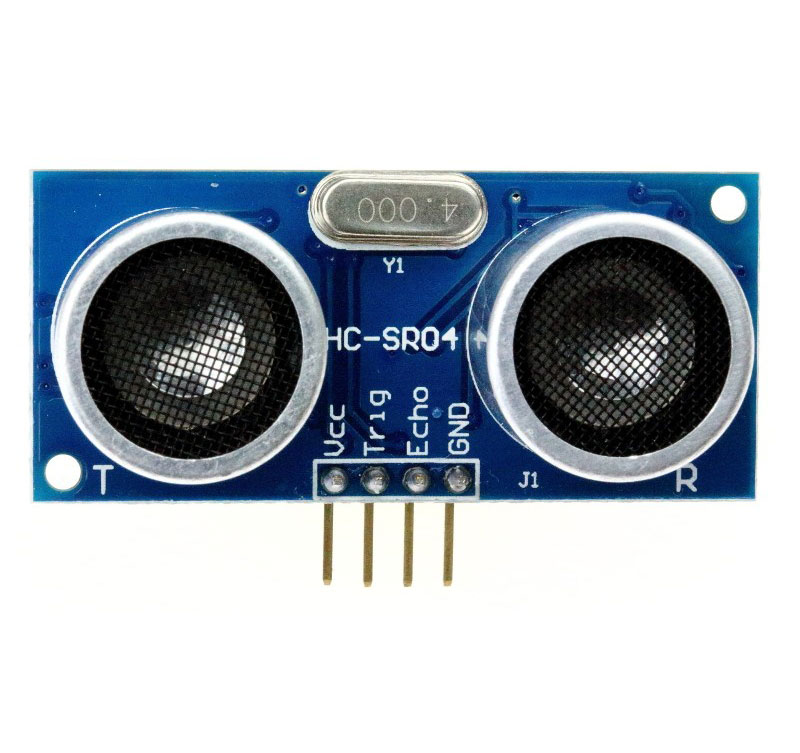
\includegraphics[scale = 0.2]{Media/Figuren/HCSR04-hardware.jpg}
    \caption{HC-SR04}
    \label{HC-SR04-component}
    \cite{HC-SR04-image-RL} 
\end{figure}
Ultrasoon sensoren zenden en ontvangen ultrasoon geluid met een frequentie van 20 kHz en bepaald met behulp van een berekening de afstand tot een object. De HC-SR04 ultrasonische sensor, te zien in figuur \ref{HC-SR04-component}\cite{HC-SR04-image-RL}, is geschikt om afstanden te meten van vier cm tot vier m door het gebruik van twee \gls{transducer}s: zender en ontvanger. De \gls{Smart-Car} moet afstanden kunnen meten tot een bepaald object, waardoor de ultrasonische sensor geschikt is voor de eisen van de opdrachtgever\cite{HC-SR04}.

De \gls{Smart-Car} beschikt over drie ultrasonische sensoren: links, rechts en voor. Door deze plaatsing van de sensoren zou de \gls{Smart-Car} door een omgeving moeten kunnen rijden en daarop kunnen reageren. 

\subsubsection{Negen Axis Sensor}
De BNO055\cite{AXIS} is een versnellingsmeter, gyroscoop, magnetometer en oriëntatie die wordt gebruikt om de oriëntatie van de \gls{Smart-Car} in de ruimte te meten. Het kan de oriëntatie van een object meten in de vorm van Euler-hoeken (roll, pitch, yaw) of als quaternion.

De BNO055\cite{AXIS} kan worden aangestuurd via een protocol. Via dit protocol kunnen verschillende configuratieparameters ingesteld worden. Momenteel wordt het alleen nog gebruikt om de \gls{Smart-Car} rechtdoor te laten rijden in de gewenste richting. 
\subsection{Actuatoren}
\subsubsection{Motoren}
Om de \gls{Smart-Car} te laten rijden worden vier motoren gebruikt. Voor het aansturen van de motoren wordt gebruik gemaakt van een \gls{motorshield}, bestaande uit twee belangrijke componenten: een 74HC595N\cite{shiftregister} \gls{shift-register} en twee L293D\cite{h-brug} \gls{H-brug} motor drivers. Het 74HC595N\cite{shiftregister} \gls{shift-register} is een seriële-in, parallel-out \gls{shift-register} met uitgangslatches, dat 8-bits extra digitale uitgangen creëert zonder extra pinnen op de \gls{microcontroller} te gebruiken. Om gegevens naar de chip te sturen, dient men seriële gegevens in te voeren op de SER-pin en SRCLK pulsen te geven aan de klok-ingang. Bij iedere puls wordt het volgende seriële bit overgezet naar het \gls{register}. Na overdracht van alle 8 bits kan de inhoud van het \gls{register} op de parallelle uitgangen worden gezien. Om de inhoud van het \gls{register} op de parallelle uitgangen te laten verschijnen, moet er een latch-puls gegeven worden, door de RCLK-pin te activeren.

De uitgangslatches van het \gls{shift-register} sturen een positief of negatief signaal naar de twee L293D\cite{h-brug} \gls{H-brug} motor drivers, waarmee de vier motoren worden aangestuurd. Door de L293D\cite{h-brug} in combinatie met een \gls{microcontroller} of andere digitale circuits te gebruiken, kan de richting en snelheid van een DC-motor worden geregeld. Het IC beschikt over vier digitale ingangen (twee voor elke motor), waarmee de motor in de gewenste richting kan worden gestuurd. Om de motor aan en uit te zetten, beschikt de L293D\cite{h-brug} tevens over één Enable-ingang per motor, die kan worden aangesloten op een \gls{PWM}-signaal om de motorsnelheid te regelen.

Het is van groot belang om de stroomsterkte van de motor en de spanning van de voeding goed te controleren en af te stemmen op de specificaties van de L293D\cite{h-brug}. Dit moet, omdat het IC een maximale stroom van 600 mA per kanaal kan leveren en is uitgerust met ingebouwde beveiligingsfuncties, zoals \gls{thermische} uitschakeling en bescherming tegen kortsluiting, wat het veilig en betrouwbaar maakt om te gebruiken in diverse toepassingen.

Om een DC-motor in één richting te laten draaien, moeten de logische waarden op IN1 en IN2 voor motor 1 respectievelijk op HIGH en LOW worden gezet. Wanneer de Enable-ingang van de motor hoog is, wordt de motor ingeschakeld en wanneer deze laag is, wordt de motor uitgeschakeld. Bovendien is er na uitgebreid onderzoek vastgesteld dat de maximale \gls{PWM}-waarde voor de motoren niet hoger dan 220 mag zijn, omdat anders de motoren kunnen doorbranden. Dankzij het gebruik van het \gls{motorshield} met de 74HC595N\cite{shiftregister} \gls{shift-register} en L293D\cite{h-brug} \gls{H-brug} motor driver kunnen de motoren op een gecontroleerde en veilige manier worden aangestuurd.

\subsubsection{Servo}
Er zit momenteel één servo op de \gls{Smart-Car}. De servo bevindt zich op de voorkant. Op deze servo is de voorste ultrasoon sensor bevestigd. De servo moet ervoor zorgen dat de ultrasoon sensor meer kan detecteren dan alleen vooruit. Dit zorgt ervoor dat de dode hoek kleiner wordt. Voor deze servo zijn verschillende versies code geschreven, dit vanwege verbeteringen en vanwege onduidelijkheden. 

\begin{lstlisting}
#include <Servo.h>
int servoPin = 10;
Servo servo;
int pos = 0;   

void setup() {
  servo.attach(10);}
void loop() {
  for (pos = 60; pos <= 120; pos += 1) { 
    servo.write(pos);              
    delay(30);}
  delay(30);
  for (pos = 120; pos >= 60; pos -= 1) {
    servo.write(pos);              
    delay(30);}}
\end{lstlisting}

De eerste code was geschreven met een library en de functie delay(). In eerste instantie is de code geschreven, om de servo heen en weer te laten zwaaien in een vloeiende beweging. Dit is gerealiseerd door eerst de library servo.h toe te voegen. vervolgens is een servo object aangemaakt, om de servo aan te kunnen sturen. Er is daarnaast een variabele int “angle” aangemaakt, welke gelijk is gesteld aan nul.  In void setup() is de servo pin gedeclareerd met behulp van de functie servo.attach. 
Dan volgt de void loop(), hierin is doormiddel van twee simpele for-loops de geleidelijke beweging gerealiseerd. Deze for-loops passen de hoek van de servo telkens aan met servo.write. Iedere keer dat de for-loop wordt doorlopen, verandert de hoek met één graden. De eerste for-loop vergroot de hoek, zolang deze kleiner of gelijk is aan 120 graden. De tweede for-loop verkleint de hoek, zolang de hoek groter of gelijk is aan 60 graden. In deze versie van de code staan in beide for-loops nog delay functies. Dit is niet ideal, want deze stoppen alle code op de Arduino Mega\cite{ArduinoMEGA} voor de duratie van de functie. 

\begin{lstlisting}
int angle;
int pwm;

void setup() {
  pinMode(10, OUTPUT);}

void loop () {
  for (angle = 60; angle <= 120; angle += 1) {
    servoPulse(10, angle);}
  for (angle = 120; angle >= 60; angle -= 1) {
    servoPulse(10, angle);}}
  
void servoPulse (int servo, int angle) {
  pwm = (angle*11) + 500;      // Convert angle to microseconds
  digitalWrite(servo, HIGH);
  delayMicroseconds(pwm);
  digitalWrite(servo, LOW);
  delay(50);                   // Refresh cycle of servo}
\end{lstlisting}

Nadat de eerste versie geschreven was, werd door een leerling van een ander groepje gezegd dat er geen library gebruikt mocht worden. Vanwege de onzekerheid over de correctheid hiervan, is de code herschreven.  Dit keer zonder library\cite{Aansturen-servo-zonder-library}. In deze versie is de pinaanduiding gedaan met “pinMode()” in plaats van “servo.attach()” en is de simpele functie “servo.write()” vervangen door de functie “servoPulse()”. In de functie “servoPulse()” is een 2e variabele int “pwm” gebruikt. Deze is gebruikt om te bepalen hoe lang de servo moet draaien om de gewenste hoek te krijgen. Hiervoor is de berekening op regel 21 van de code uitgevoerd. Door gebruik te maken van “digitalWrite()” en “delayMicroseconds()” is de servo voor de berekende duur op hoog gezet. 

\begin{lstlisting}
#include <Servo.h>
const int servoPin = 10; 
const int servoMinDegrees = 60; 
const int servoMaxDegrees = 120;
Servo servo1;
int servoPosition = servoMinDegrees;    
int servoInterval = 30; 
int servoDegrees = 1;       
int servoDegreeCounter = servoMaxDegrees;
unsigned long currentMillis = 0;    
unsigned long previousServoMillis = 0; 

void setup() {
  Serial.begin(9600);  
  servo1.write(servoPosition); 
  servo1.attach(servoPin);}

void loop() {
  currentMillis = millis();
  servoSweep();}

void servoSweep() {
    while(currentMillis - previousServoMillis >= servoInterval) {
      previousServoMillis += servoInterval;
      servoPosition = servoPosition + servoDegrees; 
      if ((servoPosition == servoMaxDegrees) || (servoPosition == servoMinDegrees)) {
      servoDegrees = - servoDegrees; 
      servoPosition = servoPosition + servoDegrees;}  
    servo1.write(servoPosition);}}
\end{lstlisting}

De 3e versie van de servo code was geschreven toen duidelijk werd dat alleen voor de motorshield geen library gebruikt mocht worden en dus voor de servo wel. Daarnaast waren de eerste twee versies niet ideaal, vanwege het gebruik van de functie “delay()”. Daarom is de code voor de servo voor een derde keer herschreven, dit keer weer met library en zonder de delay functie\cite{Functie-millis-info}. 
Zoals in de derde versie van de servo code te zien is, is dit voor elkaar gekregen door de functie “millis()” in combinatie met intervallen te gebruiken. Arduino\cite{ArduinoMEGA} houdt automatisch bij hoe lang de programmacode draait, met de functie millis() wordt deze tijd gegeven in milliseconden. Door de begintijd van een opdracht bij te houden en hier de eindtijd van de vorige opdracht of cyclus van af te trekken, kan de verstreken tijd worden bepaald. In deze versie van de servo-code is dit gedaan met de variabelen 
currentMillis en previousServoMillis. Met behulp van een variabele interval, servoInterval, kan tussen deze verstreken tijd en het interval een voorwaarde worden opgesteld, waarna of zolang iets moet gebeuren. Er is in deze versie zo een voorwaarde opgesteld en gebruikt in een while-loop, om iedere keer de servo met 1 graden te laten draaien. Wederom is dit nog de geleidelijke beweging van de servo.
Dit werkte prima als losse code, bij het combineren van de code werkte het echter niet meer. Dit zal in de toekomst dus nog verbeterd en / of aangepast moeten worden. Hierop wordt dieper ingegaan bij “Aanbevelingen”.


\subsection{Matrix}
Achterin de \gls{Smart-Car}, in het midden, bevindt zich een 8x8 matrixbord met 64 LED-punten. Het doel hiervan is om tijdens het rijden een pijl te laten zien op het matrixbord, die de richting aangeeft waarin de \gls{Smart-Car} zich beweegt. Om het bord aan te sluiten, zijn er vijf pinnen: Vcc, GND, DIN, CS en CLK. Vcc is de voedingsingang (+5V), GND geeft de grond aan (-), bij DIN wordt het signaal doorgegeven via het schuifregister en verschijnt op DOUT 16,5 klokcycli later, CS betekent dat de gegevens worden vergrendeld in de cijfer- of besturingsregisters en CLK geeft aan wanneer het leest bij elk opgaand blok signaal. Deze drie pinnen worden gecombineerd met behulp van de LedControl-library.

Gebaseerd op het doel van de codeconstructie, bestaat de code uit 10 hexadecimale combinaties, elk met een volledige richtingpijl. Deze 10 pijlen worden gedeclareerd in een reeks van sizeof en geformuleerd in een void functie. Vervolgens moet voor elke pijl, per richting,individueel worden aangegeven wanneer deze tevoorschijn moet komen. Dit kan eenvoudig worden gedaan door bij het volledige programma de gewenste pijl te selecteren met de aanroep "displayImage(IMAGES[]);". Het resultaat is een kort en efficiënt code-ontwerp dat gemakkelijk aan elk programma kan worden toegevoegd.
Dit proces is tot stand gekomen met behulp van drie codes: 
\begin{enumerate}
    \item Voorbeeldcode: dit is een replica-code die van internet is gehaald om te testen of het scherm goed werkt.
    \begin{lstlisting}
#include <MAX7219.h>
int DIN = 50;
int CS =  53;
int CLK = 51;
MAX7219 Matrix(1, DIN, CLK, CS);

// binary represention of a heart shape
const static byte HEART[8] = {
  0b01100110,
  0b10011001,
  0b10000001,
  0b10000001,
  0b01000010,
  0b00100100,
  0b00011000,
  0b00000000};

// The Letter "R"
// human-readable binary representation from left-to-right and top-to-bottom
const static byte R[8] = {
  0b00000000,
  0b01111100,
  0b01000110,
  0b01111100,
  0b01001000,
  0b01000100,
  0b01000010,
  0b00000000};

void setup() {}

void loop() {  
  // First LED in upper left Corner
  Matrix.setLed(1, 0, 0, true);
  delay(1000);
  Matrix.setLed(1, 0, 0, false);
  delay(1000);
  // Make Hearshape from array
  for(int row = 0; row <= 7; row++) {
    Matrix.setRow(1, row, HEART[row]);
    delay(100);}
  delay(1000);
  // Change Intensity to make it pulse
  for(int repeats = 0; repeats < 3; repeats++) {
    // increase intensity
    for(int i = 1; i <= 15; i++) {
      Matrix.setIntensity(1, i);
      delay(20);}
    // decrease intensity
    for(int j = 15; j >= 1; j--) {
      Matrix.setIntensity(1, j);
      delay(20);}}
  delay(1000);
  // Make Letter "R" from array
  for(int row = 0; row <= 7; row++) {
    Matrix.setRow(1, row, R[row]);
    delay(100);}
  delay(1000);
  // invert display
  Matrix.invertDisplay(1);
  delay(1000);  
  // clear display
  Matrix.clearDisplay(1);
  delay(1000);}
    \end{lstlisting}
    \item 1e code: In het eerste ontwerp van de code worden de leds aangestuurd met behulp van een binaire combinatie van getallen. Deze binaire combinatie wordt vervolgens gecombineerd met een array in een void functie. Met deze code-structuur is het gemakkelijk om de pijl op het scherm weer te geven in de actuele rijrichting van de \gls{Smart-Car}. 
    \begin{lstlisting}
void setup() {}

void loop() { 
  up();
  // letterL();}
void up() {
currentMillis = millis();  
while (currentMillis - previousMillis >= matrixdelay) {
  // Make arrowup from array
  for(int row = 0; row <= 7; row++) {
    LedControl(1, row, uparrow[row]);}  
  previousMillis += matrixdelay; //previousMillis = previousMillis + matrixdelay}}
    \end{lstlisting}
    \item Eindproduct: Omdat er 22 verschillende oriëntatie richtingen zijn, zou de combinatie van getallen in binaire vorm, het programma te lang en te complex maken. Als oplossing  is dit programma compacter gemaakt door Hexadecimale waarden te gebruiken die hetzelfde resultaat geven.
    \begin{lstlisting}
#include <LedControl.h>
const int DIN_PIN = 50;
const int CS_PIN = 53;
const int CLK_PIN = 51;

const uint64_t IMAGES[] = {
  0x081c3e0808080808,
  0x08080808083e1c08,
  0x002060ff60200000,
  0x000406ff06040000,
  0x000042e242423c00,
  0x0000424742423c00,
  0x0102040890e0e0f0,
  0x804020100907070f,
  0x0f07070910204080,
  0xf0e0e09008040201};
const int IMAGES_LEN = sizeof(IMAGES)/8;
LedControl display = LedControl(DIN_PIN, CLK_PIN, CS_PIN);

void setup() {
  display.clearDisplay(0);
  display.shutdown(0, false);
  display.setIntensity(0, 5);}

void displayImage(uint64_t image) {
  for (int i = 0; i < 8; i++) {
    byte row = (image >> i * 8) & 0xFF;
    for (int j = 0; j < 8; j++) {
      display.setLed(0, i, j, bitRead(row, j));}
    
void loop() {
  displayImage(IMAGES[i]);}
    \end{lstlisting}
\end{enumerate}
\vspace{80mm} %5mm vertical space #Dit is gedaan zodat de bluetooth afbeelding goed geplaatst wordt
\subsection{Modules}
\subsubsection{Bluetooth}\begin{figure}[h]
    \centering
    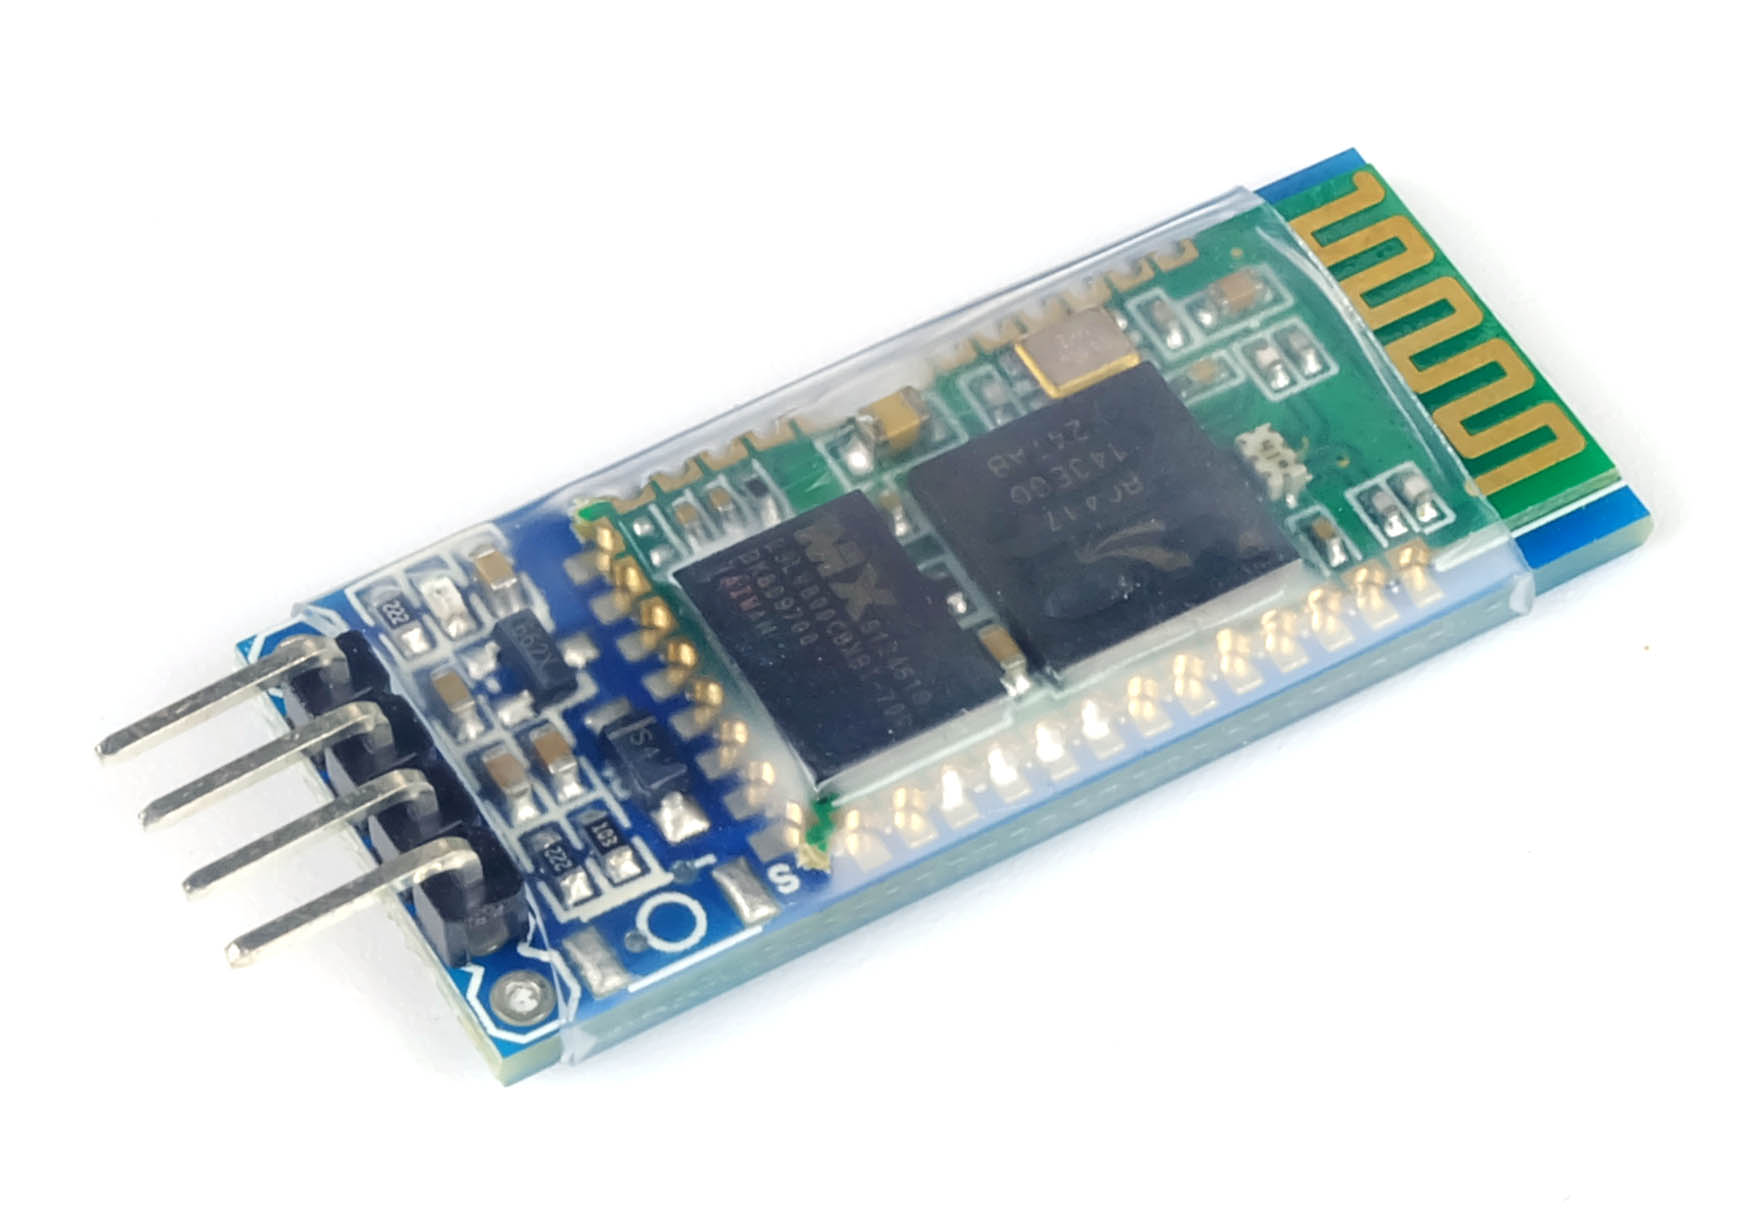
\includegraphics[scale = 0.08]{Media/Figuren/HC-05_hardware.jpg}
    \caption{HC-05}
    \label{HC-05}
    \cite{HC-05-image-fysiek-RL} 
\end{figure}

De HC-05\gls{Bluetooth} module, te zien in figuur \ref{HC-05}\cite{HC-05-image-fysiek-RL}, wordt gebruikt voor het besturen van de \gls{Smart-Car} over een afstand van maximaal tien meter. Hierbij is een applicatie gebruikt op de telefoon die door de opdrachtgever is gegeven. Het is de bedoeling dat de \gls{Smart-Car} bepaalde richtingen op kan, welke in het Programma van eisen beschreven staan. 
\subsubsection{Controller}
Tijdens de ontwikkeling van de \gls{Smart-Car} is er een controller ontworpen om een \gls{Smart-Car} aan te sturen met behulp van \gls{RF433MHZ}-chips. Verschillende componenten werden hiervoor gebruikt, waaronder een \gls{TFT-display} met een \gls{ili9341}\cite{ILI3941} IC, twee KY-023 joysticks en een ESP32\cite{ESP32} D1 MINI \gls{microcontroller}.

De ESP32\cite{ESP32} D1 MINI \gls{microcontroller} is een krachtige \gls{microcontroller} die in staat is om draadloze verbindingen te maken en complexe taken uit te voeren. Met de dubbele kern en 240 MHz rekenkracht was de ESP32\cite{ESP32} bij uitstek geschikt voor het verwerken van de gegevens van de twee KY-023 joysticks. De ingebouwde WiFi- en \gls{Bluetooth}-functionaliteit maakte het bovendien mogelijk om draadloos verbinding te maken met andere apparaten, wat tijdens de ontwikkeling van het project handig is.

Het \gls{TFT-display} met de \gls{ili9341}\cite{ILI3941} IC zorgde voor een snelle en efficiënte verwerking van de grafische weergave op het scherm. Dit gaf de mogelijkheid tot snelle en vloeiende weergave van informatie die nodig was om\gls{Smart-Car} te besturen.

De twee KY-023\cite{KY023} joysticks waren aangesloten op de ESP32\cite{ESP32} D1 MINI en na het uitlezen van de waarden, werden deze gekalibreerd en omgezet in een serieel formaat dat verzonden kon worden via de \gls{RF433MHZ}-transceiver. De combinatie van \gls{RF433MHZ} en de joysticks zorgde voor een betrouwbare en responsieve verbinding tussen de controller en de \gls{Smart-Car}, waardoor de \gls{Smart-Car} met precisie bestuurd kon worden in elke richting.

Over het algemeen waren het \gls{TFT-display} met de \gls{ili9341}\cite{ILI3941} IC en de krachtige ESP32\cite{ESP32} D1 MINI \gls{microcontroller} cruciale componenten in het ontwerp van de controller. Deze zorgden namelijk voor een vloeiende en responsieve gebruikerservaring en boden de flexibiliteit en rekenkracht die nodig was om de \gls{Smart-Car} nauwkeurig te kunnen besturen.

Daarnaast is het gebruik van de KY-023\cite{KY023} joysticks, ook een cruciaal component in het ontwerp van onze controller. De joysticks maakten het mogelijk om de \gls{Smart-Car} in elke richting te bewegen en te sturen, waardoor de controle over de \gls{Smart-Car} zeer nauwkeurig was. Dankzij de combinatie van \gls{RF433MHZ} en de joysticks kon de \gls{Smart-Car} met precisie bestuurd worden. Daarnaast zorgde de betrouwbare en responsieve verbinding tussen de controller en de \gls{Smart-Car} voor een vloeiende gebruikerservaring.

\subsection{Behuizing}
De behuizing die alles bij elkaar houdt, bestaat uit vier onderdelen:
\begin{enumerate}
\item De onderkant, een plaat, waarop de motoren en wielen met bouten en moeren zijn bevestigd.\item De boven plaat, waarop de Arduino Mega, servo en alle sensoren zijn gemonteerd.
\item De rechter zijplaat, waarop de rechter ultrasoon sensor bevestigd is.
\item De linker zijplaat, waaraan de linker ultrasoon sensor is vastgemaakt.
\end{enumerate}
De onderdelen zijn gemaakt met behulp van een 3D-printer en het materiaal PLA (Polylactic Acid). Dit is een duurzaam materiaal dat bij verhitting zacht wordt en bij afkoelen een stevig hard vorm behoudt. Dit is eenverschil ten opzichte van traditionele plastics, in dat het harder en steviger is. Om de onderdelen aan elkaar te bevestigen, zijn spacers en schroeven gebruikt, die de onderplaat en bovenplaat aan elkaar vastgeschroefd houden. De rechter en linker zijplaten zijn met schroeven aan de boven plaat gemonteerd. Deze zorgen voor een stevigeconstructie.
